%!TEX root = doc.tex
\documentclass[twoside,10pt,parskip=half,ngerman]{scrreprt}

%***********************************************************************
% include some libs
%***********************************************************************
\usepackage[utf8]{inputenc}
\usepackage{listings}
\usepackage{xcolor}
\usepackage{color}
\usepackage{fancyhdr}
\usepackage{rotating}
\usepackage{titlesec}
\usepackage{mathptmx}
\usepackage{amssymb} % checkmark
% \usepackage{helvet}
\usepackage[scaled]{uarial}
\renewcommand*\familydefault{\sfdefault} %% Only if the base font of the document is to be sans serif
\usepackage[T1]{fontenc}
\usepackage[ngerman]{babel}
\usepackage[pdfauthor={Thomas Bandixen}, pdftitle={Bachelor-/Projektarbeit FS14 Studiengang Informatik - Projekttitel}, colorlinks=true,linkcolor=black,citecolor=black,plainpages=false]{hyperref}
\usepackage{textcomp}
\usepackage[squaren]{SIunits}
\usepackage{graphicx}
\usepackage{url}
\usepackage{geometry}
\usepackage[absolute]{textpos}
\usepackage{makeidx}
\usepackage{colortbl}
\usepackage{pdflscape}
\usepackage{pdfpages}
\usepackage{tabularx}
\usepackage{lmodern}
\usepackage{longtable}
\usepackage{array}
\usepackage{float}
\usepackage{scrhack}
\usepackage{wallpaper} %\ThisTileWallPaper{}
\usepackage[super,square]{natbib} %für BibTeX Literaturverzeichnis
\usepackage{packages/usecases}
% Glossar
\usepackage{footnote}
\makesavenoteenv{description}
\usepackage[acronym,section=section]{glossaries}
\renewcommand*{\glsentryfmt}{\ifglsused{\glslabel}{\glsentryname{\glslabel}}{\glsentrydesc{\glslabel}\space(\glsentryname{\glslabel})}}
\makeglossaries

%***********************************************************************
% various styles
%***********************************************************************

%create index
\makeindex

%define pagestyle
\pagestyle{fancy}

%use sans-serif font
%\renewcommand{\familydefault}{\sfdefault}

%define page margin
\geometry{a4paper, top=30mm, left=30mm, right=30mm, bottom=30mm,headsep=10mm,footskip=10mm}

%textpos parameter
\setlength{\TPHorizModule}{30mm}
\setlength{\TPVertModule}{\TPHorizModule}
\textblockorigin{10mm}{10mm} % start everything near the top-left corner
\setlength{\parindent}{0pt}

%horizontal lines for titlepage
\newcommand{\HRule}{\rule{\linewidth}{0.5mm}}

%reference to source items inlc source number
\newcommand{\srcref}[1]{\nameref{src:#1} \cite{#1}}

%header / footer
\renewcommand{\headrulewidth}{0.3pt}
\renewcommand{\footrulewidth}{0.3pt}

\fancyhead[LO,RE]{} %clear headings for contents
\fancyhead[RO,LE]{\nouppercase{\rightmark}} %right odd pages and left even pages
\fancyhead[LO,RE]{\MakeUppercase{\leftmark}} %left odd pages and right even pages
\fancyfoot[LE,RO]{\thepage} %page numbering
\fancyfoot[C]{} %clear centered page numbering

%define some colors
\definecolor{gray}{rgb}{0.95,0.95,0.95}
\definecolor{darkgray}{rgb}{0.4,0.4,0.4}
%listing colors
\definecolor{lgray}{RGB}{250,250,250}
\definecolor{lgreen}{RGB}{63,127,95}
\definecolor{lred}{RGB}{127,0,85}
\definecolor{lblue}{RGB}{42,0,255}

%***********************************************************************
% listing
%***********************************************************************

\lstset{
		basicstyle=\small\ttfamily,
		frame=single,
		numbers=left,
		numberstyle=\tiny,
		%firstnumber=auto,
		numberblanklines=true,
		captionpos=b,
		extendedchars=true,
		float=ht,
		showtabs=false,
		tabsize=2,
		showspaces=false,
		showstringspaces=false,
		breaklines=true,
		%prebreak=\Righttorque,
		backgroundcolor=\color{lgray},
		keywordstyle=\color{lred}\bfseries,
		commentstyle=\color{lgreen}\ttfamily,
%		morekeywords={printstr, printhexln},
		stringstyle=\color{lblue},
		xleftmargin=0.5cm,
		xrightmargin=0.5cm
}

\lstloadlanguages{[Sharp]C}
%\lstdefinestyle{sharpc}{language=[Sharp]C, frame=lr} %, rulecolor=\color{blue!80!black}

%\lstdefinelanguage{xc}{
%     keywords={printstr, printhexln, attributes, class, classend, do, empty, endif, endwhile, fail, function, functionend, if, implements, in, inherit, inout, not, of, operations, out, return, set, then, types, while, use},
%     keywordstyle=\color{lred}\bfseries,
%     ndkeywords={},
%     ndkeywordstyle=\color{yellow}\bfseries,
%     identifierstyle=\color{black},
%     sensitive=false,
%     comment=[l]{//},
%     commentstyle=\color{lgreen}\ttfamily,
%     string=[l]{"},
%     stringstyle=\color{lblue}\ttfamily
%  }


\begin{document}
\newglossaryentry{zhaw}{name=ZHAW,description=Zürcher Hochschule für Angewandte Wissenschaften}

\bibliographystyle{plainnat}

\title{PA/BA \LaTeX Vorlage} % In header.tex nachtragen
\author{Thomas Bandixen}

\begin{titlepage}

% Logo
\ThisTileWallPaper{\paperwidth}{\paperheight}{images/logos/SoE.pdf} % {images/logos/*.pdf}

\begin{minipage}[b]{0.117\textwidth}
\hskip 0.05cm
\end{minipage}
\begin{minipage}[b]{0.91\textwidth}
\begin{tiny}.\end{tiny}\vskip 2.8cm
	{\huge
	
	% Projekt Name (max. 2 Zeilen)
	\textbf{\underline{Bachelor-/Projektarbeit}}\\
	\textbf{\underline{FS14 Studiengang Informatik}}
	
	% Projekt Titel (max. 4 Zeilen)
	Titel der Arbeit
	\vskip 0.5cm}
	
	\begin{minipage}[b]{0.27\textwidth}
	\hrule\vskip 0.5cm
		\textbf{Autoren}\\
		\\
	\end{minipage}
	\begin{minipage}[b]{0.03\textwidth}
	\hskip 0.5cm
	\end{minipage}
	\begin{minipage}[b]{0.7\textwidth}
	\hrule\vskip 0.5cm
		Vorname Name\\
		Vorname Name\\
	\end{minipage}
	
	\begin{minipage}[b]{0.27\textwidth}
	\hrule\vskip 0.5cm
		\textbf{Hauptbetreuung}\\
		\\
	\end{minipage}
	\begin{minipage}[b]{0.03\textwidth}
	\hskip 0.5cm
	\end{minipage}
	\begin{minipage}[b]{0.7\textwidth}
	\hrule\vskip 0.5cm
		Vorname Name\\
		Vorname Name\\
	\end{minipage}
	
	\begin{minipage}[b]{0.27\textwidth}
	\hrule\vskip 0.5cm
		\textbf{Nebenbetreuung}\\
		\\
	\end{minipage}
	\begin{minipage}[b]{0.03\textwidth}
	\hskip 0.5cm
	\end{minipage}
	\begin{minipage}[b]{0.7\textwidth}
	\hrule\vskip 0.5cm
		Vorname Name\\
		Vorname Name\\
	\end{minipage}
	
	\begin{minipage}[b]{0.27\textwidth}
	\hrule\vskip 0.5cm
		\textbf{Industriepartner}\\
		\\
	\end{minipage}
	\begin{minipage}[b]{0.03\textwidth}
	\hskip 0.5cm
	\end{minipage}
	\begin{minipage}[b]{0.7\textwidth}
	\hrule\vskip 0.5cm
		Firmenname\\
		\\
	\end{minipage}
	
	\begin{minipage}[b]{0.27\textwidth}
	\hrule\vskip 0.5cm
		\textbf{Externe Betreuung}\\
		\\
	\end{minipage}
	\begin{minipage}[b]{0.03\textwidth}
	\hskip 0.5cm
	\end{minipage}
	\begin{minipage}[b]{0.7\textwidth}
	\hrule\vskip 0.5cm
		Vorname Name\\
		Vorname Name\\
	\end{minipage}
	
	\begin{minipage}[b]{0.27\textwidth}
	\hrule\vskip 0.5cm
		\textbf{Datum}
	\end{minipage}
	\begin{minipage}[b]{0.03\textwidth}
	\hskip 0.5cm
	\end{minipage}
	\begin{minipage}[b]{0.7\textwidth}
	\hrule\vskip 0.5cm
		01.01.2011
	\end{minipage}
\end{minipage}
\vskip 0.5cm


\textcolor{darkgray}{
Bitte füllen Sie das Titelblatt aus und berücksichtigen Sie Folgendes:\\
 -> Bitte auf keinen Fall Schriftart und Schriftgrösse ändern. Text soll lediglich überschrieben werden!\\
 -> Bitte pro Tabellenzeile max. 4 Textzeilen!\\
\\
•	Vorlage: Haben Sie die richtige Vorlage gewählt? Logo Institut/Zentrum\\
•	Titel: Fügen Sie Ihren Studiengang direkt nach dem Wort „Bachelorarbeit“ ein (max. 2 Zeilen).\\
•	Titel der Arbeit: Überschreiben Sie den Lauftext mit dem Titel Ihrer Arbeit (max. 4 Zeilen).\\
•	Autoren: Tragen Sie Ihre Vor- und Nachnamen ein (alphabetisch nach Name).\\
•	Betreuer: Tragen Sie Ihren Betreuer / Ihre Betreuer ein (alphabetisch nach Name).\\
•	Ohne Nebenbetreuung, Industriepartner oder externe Betreuung, ganze Tabellenzeile löschen.\\
•	Datum: Aktuelles Datum eintragen.\\
•	Am Schluss löschen Sie den ganzen Beschrieb (grau) und speichern das Dokument als pdf. ab.
}

\end{titlepage}

\setcounter{page}{1}
%!TEX root = ../doc.tex
\thispagestyle{empty}
\chapter*{Zusammenfassung}
\label{sec:Zusammenfassung}
\textcolor{darkgray}{
  Zusammenfassung
}

\chapter*{Vorwort}
\label{sec:Vorwort}

\textcolor{darkgray}{
  Stellt den persönlichen Bezug zur Arbeit dar und spricht Dank aus.
}


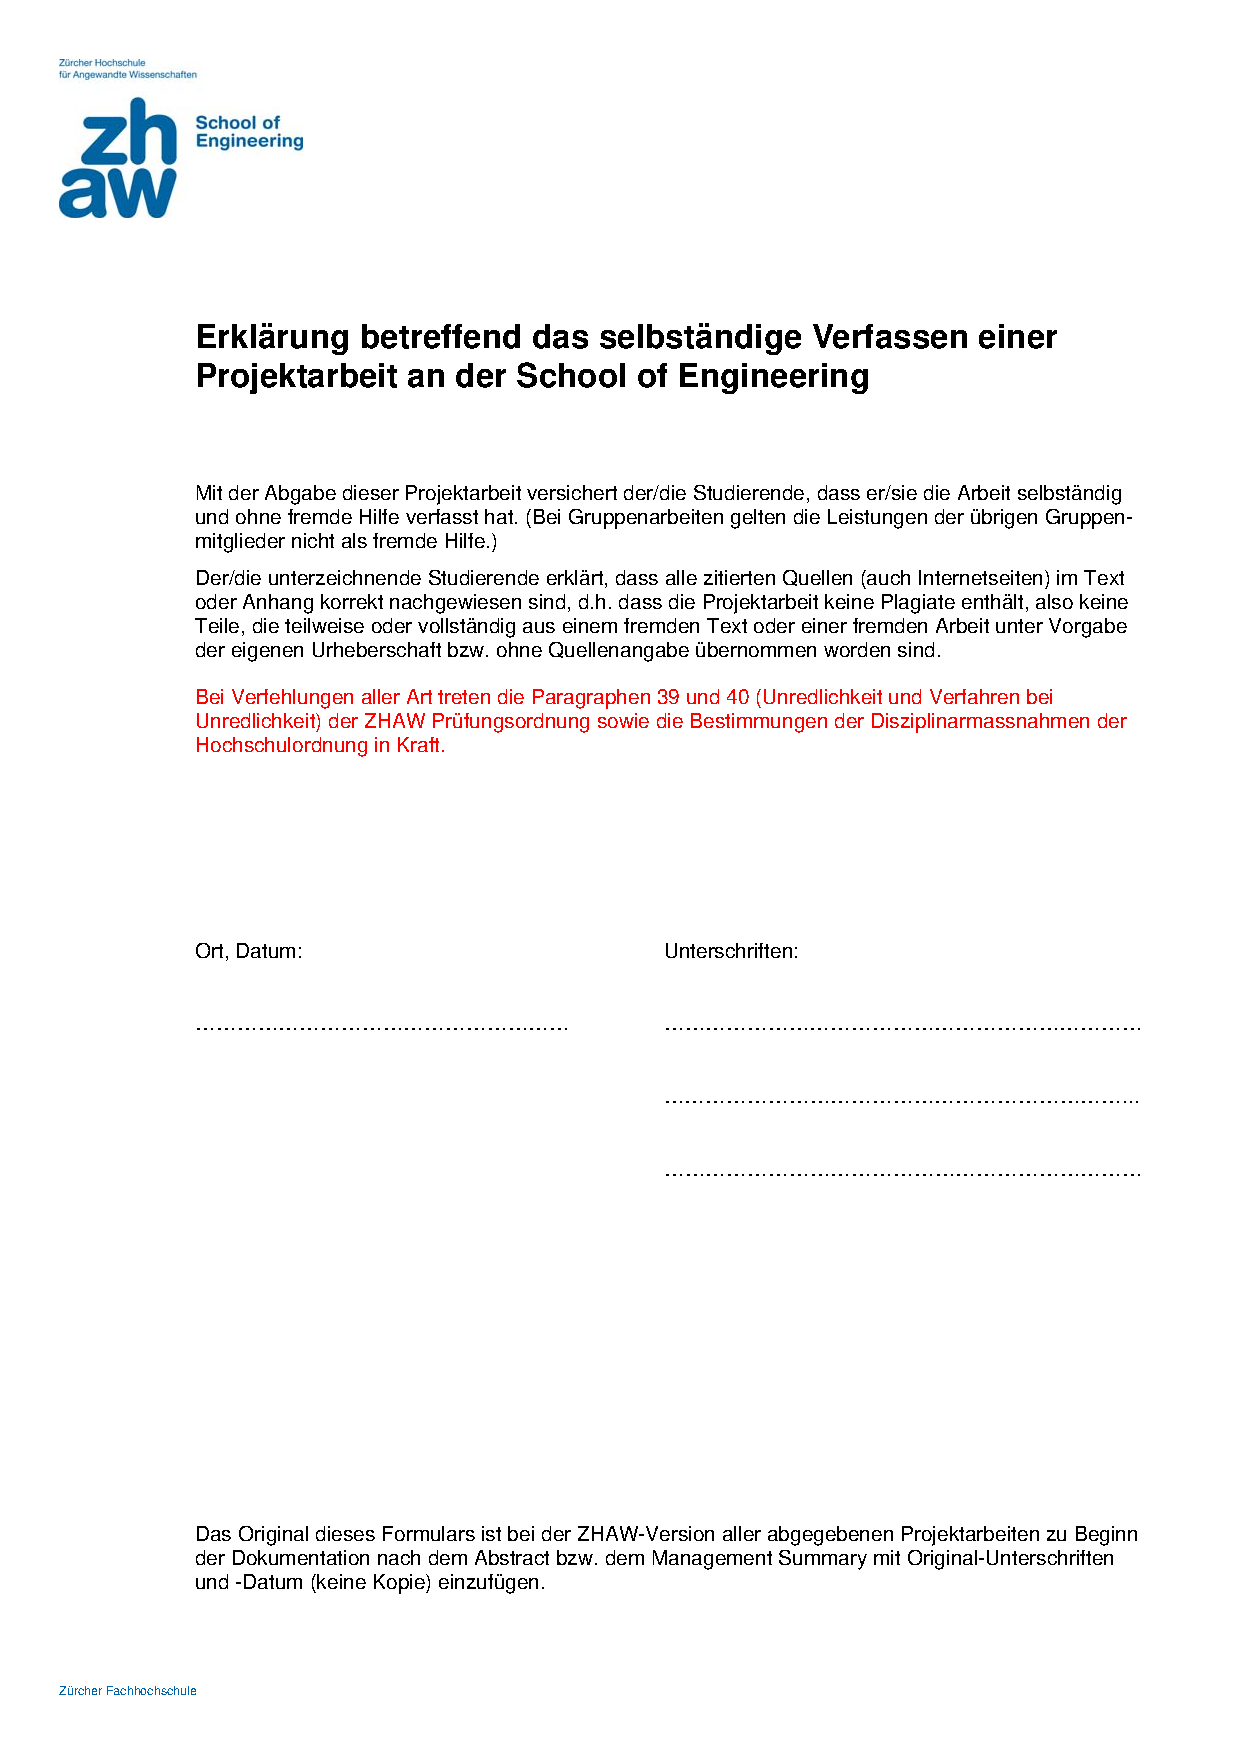
\includepdf{images/Erklaerung_PA.pdf} % Entsprechendes auskommentieren
% 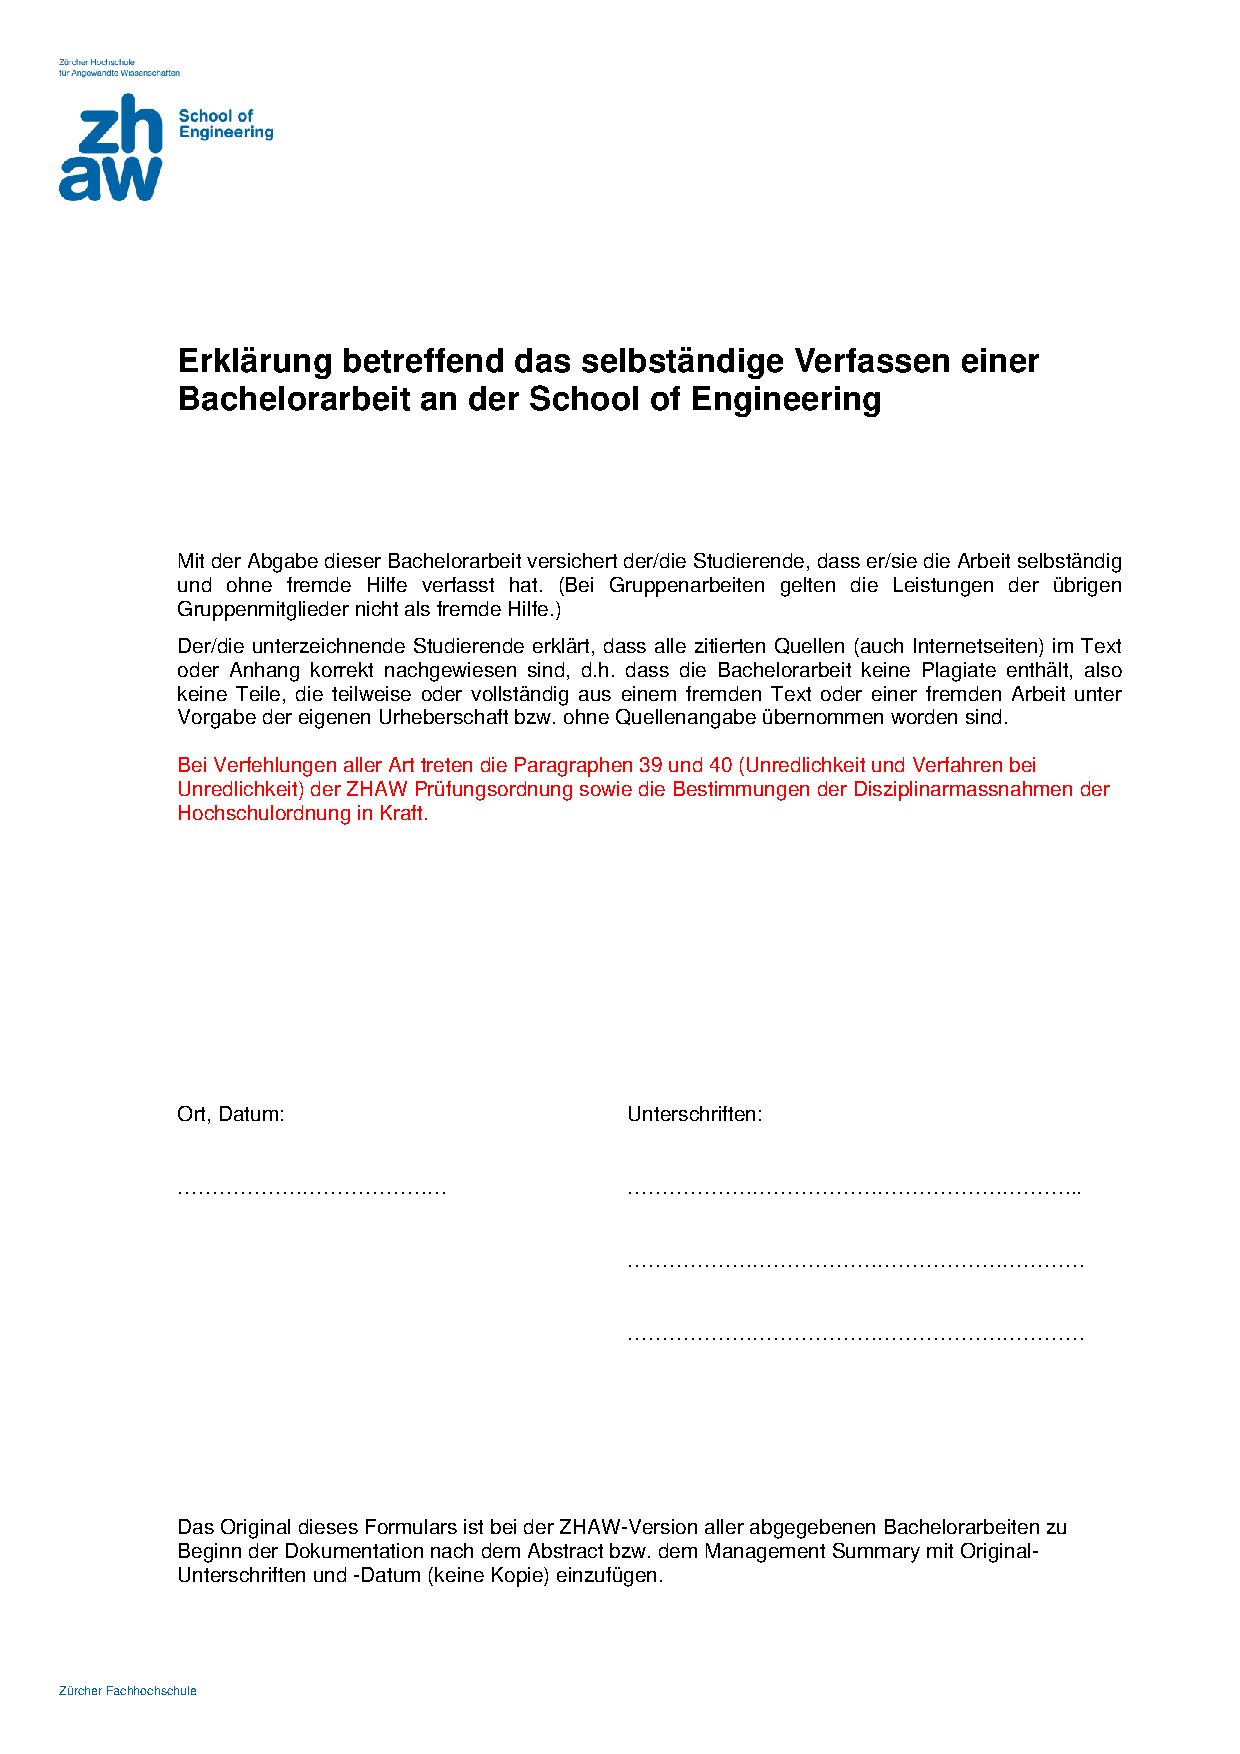
\includepdf{images/Erklaerung_BA.pdf}
% \newpage

%Inhaltsverzeichnis
\tableofcontents
\newpage

%\textbf{}
%\setcounter{page}{1}
%\pagenumbering{arabic}

%!TEX root = ../doc.tex
\chapter{Einleitung}
\label{sec:Einleitung}

\section{Ausgangslage}
\label{sec:Ausgangslage}

\textcolor{darkgray}{
  \begin{itemize}
  \item Nennt bestehende Arbeiten/Literatur zum Thema -> Literaturrecherche
  \item Stand der Technik: Bisherige Lösungen des Problems und deren Grenzen
  \item (Nennt kurz den Industriepartner und/oder weitere Kooperationspartner und dessen/deren Interesse am Thema Fragestellung)
  \end{itemize}
}

\section{Zielsetzung / Aufgabenstellung / Anforderungen}
\label{sec:ZielsetzungAufgabenstellungAnforderungen}

\textcolor{darkgray}{
  \begin{itemize}
  \item Formuliert das Ziel der Arbeit
  \item Verweist auf die offizielle Aufgabenstellung des/der Dozierenden im Anhang
  \item (Pflichtenheft, Spezifikation)
  \item (Spezifiziert die Anforderungen an das Resultat der Arbeit)
  \item (Übersicht über die Arbeit: stellt die folgenden Teile der Arbeit kurz vor)
  \item (Angaben zum Zielpublikum: nennt das für die Arbeit vorausgesetzte Wissen)
  \item (Terminologie: Definiert die in der Arbeit verwendeten Begriffe)
  \end{itemize}
}
%!TEX root = ../doc.tex
\chapter{Theoretische Grundlagen}
\label{sec:TheoretischeGrundlagen}
 % (2. Theoretische Grundlagen)
%!TEX root = ../doc.tex
\chapter{Vorgehen / Methoden}
\label{sec:VorgehenMethoden}

\textcolor{darkgray}{
  \begin{itemize}
  \item (Beschreibt die Grundüberlegungen der realisierten Lösung (Konstruktion/Entwurf) und die Realisierung als Simulation, als Prototyp oder als Software-Komponente)
  \item (Definiert Messgrössen, beschreibt Mess- oder Versuchsaufbau, beschreibt und dokumentiert Durchführung der Messungen/Versuche)
  \item (Experimente)
  \item (Lösungsweg)
  \item (Modell)
  \item (Tests und Validierung)
  \item (Theoretische Herleitung der Lösung)
  \end{itemize}
}

\section{Verwendete Software}
\label{sec:VerwendeteSoftware}
Für die vorliegende Arbeit wurden die unten aufgeführten Programme eingesetzt.

\subsection*{Arbeitsumgebung}\label{wintool}
\begin{itemize}
	\item Microsoft Windows 8 developer preview
\end{itemize}

\subsection*{Virtual Machine}\label{vm}
\begin{itemize}
	\item Oracle VM VirtualBox, Version 3.2.10
\end{itemize}

\subsection*{CAD Catia}\label{catia}
\begin{itemize}
	\item CATIA, Version 5.19 (in VirtualBox)
\end{itemize}

\subsection*{Dokumentation}\label{dokutools}
\begin{itemize}
  \item \LaTeX{} mit TeXnicCenter 2.02 Stable (64 bit)\cite{TeXnicCenter:2014:Online}
	\item proTeXt mit TexMakerX 2.1 (SVN 1774), \href{http://www.latex-project.org/ftp.html}{latex-project.org}
	\item Microsoft Visio 2007
	\item Adobe Acrobat 8 Professional 8.1.6
\end{itemize}
 % Vorgehen / Methoden
%!TEX root = ../doc.tex
\chapter{Resultate}
\label{sec:Resultate}

\textcolor{darkgray}{
  \begin{itemize}
  \item (Zusammenfassung der Resultate)
  \end{itemize}
}

\chapter{Diskussion und Ausblick}
\label{sec:DiskussionUndAusblick}

\textcolor{darkgray}{
  \begin{itemize}
  \item Bespricht die erzielten Ergebnisse bezüglich ihrer Erwartbarkeit, Aussagekraft und Relevanz
  \item Interpretation und Validierung der Resultate
  \item Rückblick auf Aufgabenstellung, erreicht bzw. nicht erreicht
  \item Legt dar, wie an die Resultate (konkret vom Industriepartner oder weiteren Forschungsarbeiten; allgemein) angeschlossen werden kann; legt dar, welche Chancen die Resultate bieten
  \end{itemize}
} % Diskussion und Ausblick

\chapter{Verzeichnisse}
\label{sec:Verzeichnisse}
\addcontentsline{toc}{section}{Literaturverzeichnis}
\bibliography{BibTeX/literatur}
\listoffigures
\addcontentsline{toc}{section}{Abbildungsverzeichnis}
\listoftables
\addcontentsline{toc}{section}{Tabellenverzeichnis}
%!TEX root = ../doc.tex
\chapter*{Glossar}
\label{sec:Glossar}
\addcontentsline{toc}{section}{Abkürzungsverzeichnis}\label{cha:abkürzungsverzeichnis}

In diesem Abschnitt werden Abkürzungen und Begriffe kurz erklärt.
\setglossarystyle{altlistgroup}
\printglossary[title=]


\lstlistoflistings
\addcontentsline{toc}{section}{Listingverzeichnis}

%!TEX root = ../doc.tex
\pagenumbering{Roman}

\appendix
\chapter{Anhang}
\label{sec:Anhang}

\section{Projektmanagement}\label{projektmanagement}

\textcolor{darkgray}{
  \begin{itemize}
  \item Offizielle Aufgabenstellung, Projektauftrag
  \item (Zeitplan)
  \item (Besprechungsprotokolle oder Journals)
  \end{itemize}
}

\section{Weiteres}
\label{sec:Weiteres}

\textcolor{darkgray}{
  \begin{itemize}
  \item CD mit dem vollständigen Bericht als pdf-File inklusive Film- und Fotomaterial
  \item (Schaltpläne und Ablaufschemata)
  \item (Spezifikationen u. Datenblätter der verwendeten Messgeräte und/oder Komponenten)
  \item (Berechnungen, Messwerte, Simulationsresultate)
  \item (Stoffdaten)
  \item (Fehlerrechnungen mit Messunsicherheiten)
  \item (Grafische Darstellungen, Fotos)
  \item (Datenträger mit weiteren Daten (z.B. Software-Komponenten) inkl. Verzeichnis der auf diesem Datenträger abgelegten Dateien)
  \item (Softwarecode)
  \end{itemize}
}


\end{document}
